\documentclass[a4paper,11pt]{article}
\input{/home/tof/Documents/Cozy/latex-include/preambule_lua.tex}
\newcommand{\showprof}{show them}  % comment this line if you don't want to see todo environment
\fancyhead[L]{TITRE}
\newdate{madate}{10}{09}{2020}
\fancyhead[R]{\displaydate{madate}} %\today
\fancyfoot[L]{~\\Christophe Viroulaud}
\fancyfoot[C]{\textbf{Page \thepage}}
\fancyfoot[R]{\includegraphics[width=2cm,align=t]{/home/tof/Documents/Cozy/latex-include/cc.png}}
\usepackage{tikz}

\begin{document}
\begin{Form}
\begin{exo}
Une liste doublement chaînée occupe davantage d'espace en mémoire. Cependant elle possède des avantages pour l'insertion d'un élément.
\begin{figure}[!h]
\centering
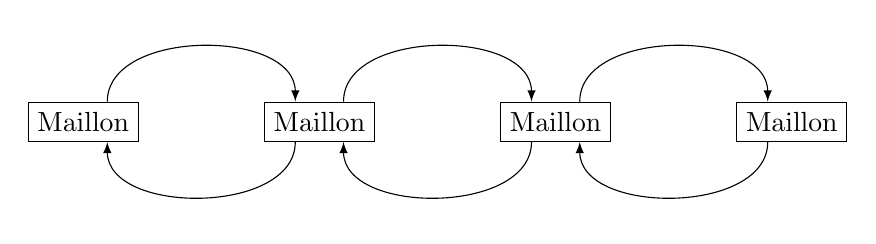
\begin{tikzpicture}[scale=0.5]
\node[draw,minimum width=1cm, minimum height=0.5cm] (1) at (-6,0) {Maillon};
\node[draw,minimum width=1cm, minimum height=0.5cm] (2) at (0,0) {Maillon};
\node[draw,minimum width=1cm, minimum height=0.5cm] (3) at (6,0) {Maillon};
\node[draw,minimum width=1cm, minimum height=0.5cm] (4) at (12,0) {Maillon};

\draw[->,>=latex] (1.40) to[out=90,in=90] (2.140);
\draw[->,>=latex] (2.40) to[out=90,in=90] (3.140);
\draw[->,>=latex] (3.40) to[out=90,in=90] (4.140);
\draw[->,>=latex] (4.220) to[out=270,in=270] (3.320);
\draw[->,>=latex] (3.220) to[out=270,in=270] (2.320);
\draw[->,>=latex] (2.220) to[out=270,in=270] (1.320);

\end{tikzpicture}
\captionof{figure}{Liste doublement chaînée}
\end{figure}
\begin{enumerate}
\item En s'appuyant sur la figure construire une classe \emph{Maillon} permettant de créer une liste doublement chaînée.
\item Construire alors la classe \emph{Liste\_double}.
\end{enumerate}
\end{exo}
\end{Form}
\end{document}